
\chapter{Introduction}
The main objective for this report is to propose a \acf{LNA} front-end for extracellular\footnote{\emph{extracellular} means "outside the cell"} in-vito\footnote{\emph{in-vivo} is Latin for "within the living"}
neural signal recording electrodes, as well as to research what requirements can be considered critical in achieving such a design. As a natural consequence of the main objective, the project - which this report is a
product of - will explore the usage of \acs{CMOS} technology in neural recording systems. Any findings produced can therefore be used as a preliminary for further research in the authors upcoming graduate thesis. 
Thus, some basic elaborations on where the design can potentially be situated in a complete \acf{BMI} - such as a bio-medical \acs{IC} or a neuro \acs{MEMS} array with fully integrated electronics, will be undergone. \\*

The rest of this chapter will describe the motivation for initiating this project, provide a rudimentary overview of past work in this area, mention outcomes of the project, and outline the structure of the rest of the report.

\section{Motivational Background}
Technological advances towards a type of electromechanical or biomedical augmentation of the human body which remedies,
    improves or maybe even grants the user a new set of abilities are intriguing thoughts for anyone with a little \emph{cyberpunk} in them. There is still
    quite a long way before any such leaps in technology are possible. However, forcing oneself into more pragmatical ways of thinking; there is no doubt that demands for technologies enabling scientists and clinicians to record neural activity from a large number of neurons in a brain is continuously rising. Namely collecting high temporal and spatial resolution neural data from micromachined multielectrode arrays is something that can be regarded standard practice in basic neuroscientifical research \cite{harrison2003low}. Such research is starting to enable medical, as well as neuroprosthetic applications, and we see that neural recordings can provide scientific insight into the neural correlates of cognitive, sensory and motor processes \cite{miller2007spectral,chang2010categorical,gunduz2011neural}. Experiments and clinical trials with primates - both human \cite{hochberg2006neuronal} and non-human \cite{wessberg2000real}, as subjects have shown that data directly derived from signals - namely action and \acl{LFP}s (which are to be discussed in chapter \ref{chap:two}), can be used to control robotic prosthetics.

    In the efforts to implement wholly implantable devices for neural recording purposes, \acf{MEMS} electrode arrays can be complimented with \acf{CMOS} \acl{IC}s in such a way that one achieves parallel stand-alone \acs{BMI}s with on-board wireless data and power transfer, as well as \acs{ADC}s and a processor \cite{najafi1986implantable,wise2004wireless,olsson2005three}. The continuously improving resolutions of \acs{MEMS} arrays have enabled simultaneous recording of large neuron populations with spatial resolutions down to a single cell activity from populations of neurons \cite{kipke2003silicon}.

    Studies such as the ones mentioned have shown a promising future for developing \acs{BMI}s that have practical use for humans. But to reach that point in the future where such systems can be implanted in-vito in humans and function symbiotically with them in their everyday activities, many challenges must be overcome. 
%--------------------------figure-------------------------------------------------------------------
    \begin{figure}
	\centering
	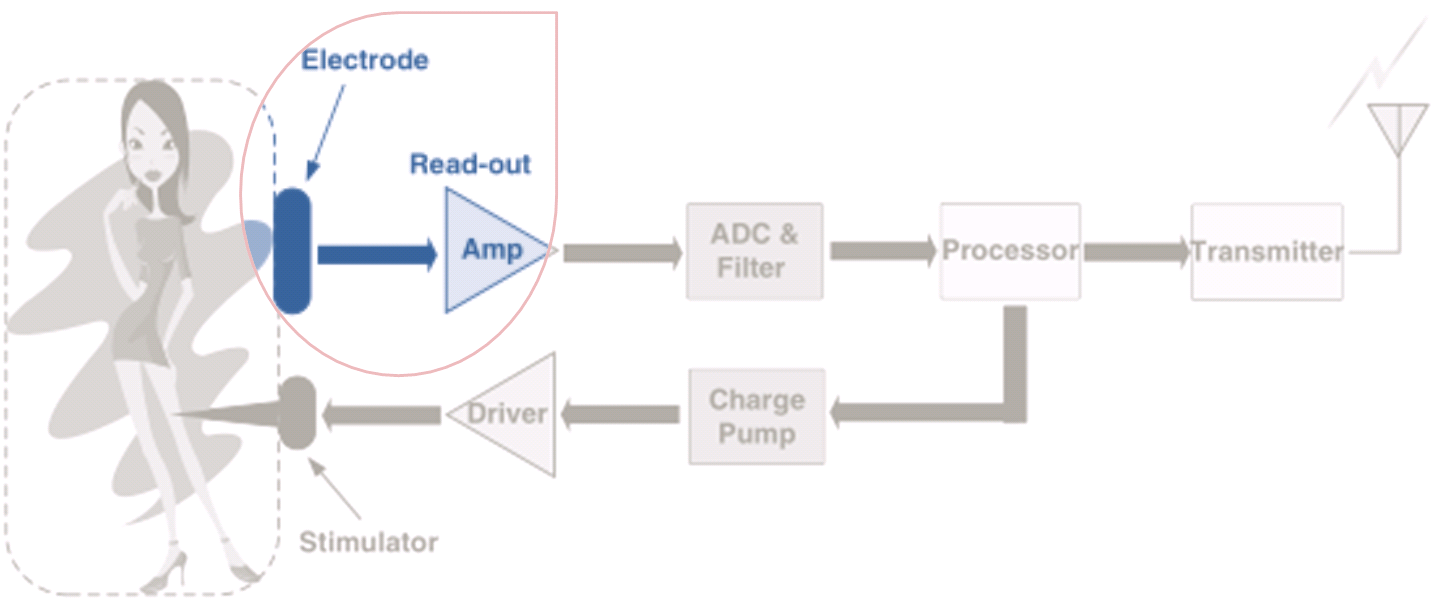
\includegraphics[scale=.4]{images/block-bio-medical-subsystem.png}
	\caption{\texttt{\footnotesize{typical architecture of bio-medical \acs{IC} subsystem \cite{yoo2011biomedical-cmos}}}}
	\label{fig:block-arch-biomedical-subsystem}
    \end{figure}       
%--------------------------END-------------------------------------------------------------------
%--------------------------figure-------------------------------------------------------------------  
\begin{wrapfigure}{r}{5.7cm}
  \vspace{-20pt}
  \caption{\texttt{\footnotesize{block diagram of a wireless neural recording device}}}
  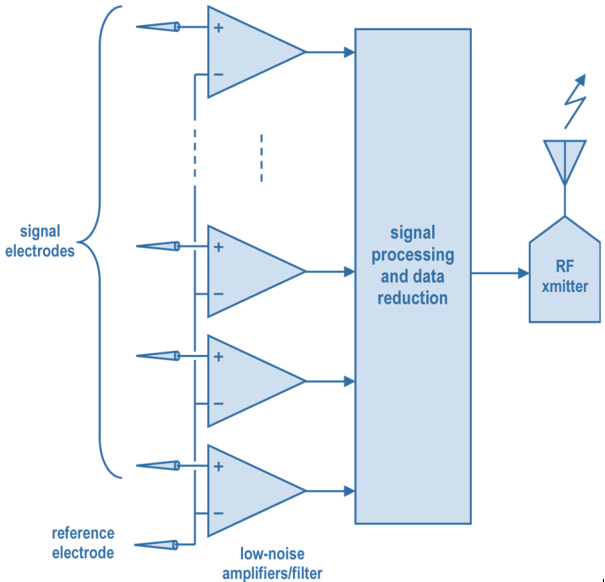
\includegraphics[width=5.7cm]{images/block-wirelss-neural-rec-dev.png}
  \vspace{-30pt} 
  \label{fig:block-neural-recording-dev}
\end{wrapfigure} 
%--------------------------END------------------------------------------------------------------- 
    Even though we are limited to propose a preliminary design for a \acl{LNA} front-end for neuro-probes with a type of platinum/iridium based electrodes, we will explore requirements to make the design compatible for integration in a complete in-vito \acl{BMI} which utilizes a \acs{MEMS} electrode array based transducer. The research in this area will ideally continue in the authors upcoming graduate thesis. A block diagram illustrating our focal point in a complete biomedical \acs{IC} - which also has an interface for stimulation, is shown in figure \ref{fig:block-arch-biomedical-subsystem}. Also, a block diagram depicting the principle for a multielectrode wireless neural interface is given in figure \ref{fig:block-neural-recording-dev}.
  
\section{Past Work}
    %refer MIT thesis
There is much literature describing both conceptual and physical implementations neural recording systems with varying degrees of practical usability. derpa derp...%TODO:

\section{Summary of Authors Contributions}
  \begin{itemize} 
    \item nada
    \item nuthin'
  \end{itemize}

\section{Report Outline}
The report is organized in the following manner:
  \begin{itemize}
    \item \textbf{Chapter 2} briefly presents the motivational background for neural recording before digging into the relevant theory needed to understand the design 
		  itself as well as eventual limitations and difficulties in realizing the best possible specifications. 
		  It also provides a basic theoretical understanding of the neural recording principles from an electronic designers point of view - namely how \acs{LNA} to interface
		  with intercranial electrodes.
    \item \textbf{Chapter 3} TODO
    \item \textbf{Chapter 4} TODO
  \end{itemize}
 